\documentclass[10pt,a4paper]{article}
\usepackage[utf8]{inputenc}
\usepackage[francais]{babel}
\usepackage[T1]{fontenc}
\usepackage{amsmath}
\usepackage{amsfonts}
\usepackage{amssymb}
\usepackage{graphicx}
\usepackage{lmodern}
\usepackage{listings}
\usepackage{color}
\usepackage{qtree}
\definecolor{mygreen}{rgb}{0,0.6,0}
\definecolor{mygray}{rgb}{0.5,0.5,0.5}
\definecolor{mymauve}{rgb}{0.58,0,0.82}

\lstset{ %
  backgroundcolor=\color{white},   % choose the background color; you must add \usepackage{color} or \usepackage{xcolor}
  basicstyle=\footnotesize,        % the size of the fonts that are used for the code
  breakatwhitespace=false,         % sets if automatic breaks should only happen at whitespace
  breaklines=true,                 % sets automatic line breaking
  captionpos=b,                    % sets the caption-position to bottom
  commentstyle=\color{mygreen},    % comment style
  deletekeywords={...},            % if you want to delete keywords from the given language
  escapeinside={\%*}{*)},          % if you want to add LaTeX within your code
  extendedchars=true,              % lets you use non-ASCII characters; for 8-bits encodings only, does not work with UTF-8
  frame=single,                    % adds a frame around the code
  keepspaces=true,                 % keeps spaces in text, useful for keeping indentation of code (possibly needs columns=flexible)
  keywordstyle=\color{blue},       % keyword style
  language=Java,                 % the language of the code
  morekeywords={*,...},            % if you want to add more keywords to the set
  numbers=left,                    % where to put the line-numbers; possible values are (none, left, right)
  numbersep=5pt,                   % how far the line-numbers are from the code
  numberstyle=\tiny\color{mygray}, % the style that is used for the line-numbers
  rulecolor=\color{black},         % if not set, the frame-color may be changed on line-breaks within not-black text (e.g. comments (green here))
  showspaces=false,                % show spaces everywhere adding particular underscores; it overrides 'showstringspaces'
  showstringspaces=false,          % underline spaces within strings only
  showtabs=false,                  % show tabs within strings adding particular underscores
  stepnumber=2,                    % the step between two line-numbers. If it's 1, each line will be numbered
  stringstyle=\color{mymauve},     % string literal style
  tabsize=4,                       % sets default tabsize to 2 spaces
  title=\lstname                   % show the filename of files included with \lstinputlisting; also try caption instead of title
}
\usepackage[left=2cm,right=2cm,top=2cm,bottom=2cm]{geometry}


\date{7 novembre 2014}
\author{Groupe 2.2}
\title{Produit Mission 4}

\begin{document}
\maketitle

\section*{Question 1 : Zacharie Kerger}

Les clés mémorisées dans les noeuds d'un arbre binaire de recherche ne doivent pas être forcément des nombres. En effet, du moment que l'on a une notion d'ordre entre les différentes clés, c'est suffisant.  Autrement dit, tant qu'une classe implémente l'interface \emph{Comparable}, les objets de cette même classe peuvent servir de clés.\\
\newline
Pour énumérer toutes les clés en ordre croissant, il faut effectuer un parcours préfixe de l'arbre qui a une complexité temporelle $\Theta(n)$ où n représente le nombre total de noeuds. On obtient cette complexité puisque l'on va visiter chaque noeud de l'arbre sans exception.\\
\newline
TO DO

\section*{Question 2 : Arnaud Dethise}

	Un arbre binaire de recherche possède deux avantages par rapport à une HashMap :
	\begin{itemize}
		\item Il est trié.
		\item Il ne contient pas de "case" vide et pas de problème de \textit{load factor}.
	\end{itemize}
	On peut donc, par exemple, facilement récupérer tous les éléments ou une séquence d'élément.
	
	Il n'a en revanche pas vraiment d'avantage sur une skip list, mis à part le fait qu'il soit plus simple et non-probabiliste.
	
	\vspace{0.5cm}
	La forme de l'arbre et, par conséquent, l'efficacité des recherches à l'intérieur de celui-ci dépend de l'ordre dans lequel les entrées sont introduites.
	
	\begin{figure}[!h]
	\begin{minipage}[b]{0.45\linewidth}
		\Tree [.1 ~ [.2 ~ 3 ] ]
		\caption{Clés introduites : 1, 2, 3}
		\label{order_keys_ex1}
	\end{minipage}
	\hspace{0.5cm}
	\begin{minipage}[b]{0.45\linewidth}
		\Tree [.2 1 3 ]
		\caption{Clé introduites : 2, 1, 3}
		\label{order_keys_ex2}
	\end{minipage}
	\end{figure}
	
	En revanche, la nécessité de garder l'arbre trié lorsque l'on supprime une clé, imposant parfois de remonter un nœud de plusieurs niveaux, fait que l'ordre de suppression d'une série de nœuds n'a pas d'importance sur sa forme après que toutes les clés de la série aient été supprimées.
	
	\vspace{0.5cm}
	En supposant que lorsque l'on veut insérer une clé ayant la même valeur qu'un nœud externe, on l'ajoute systématique du même côté, la structure résultante sera la suivante :
	
	\begin{figure}[!h]
		\Tree [.A [.A [.A [.A ] ~ ] ~ ] ~ ]
		\caption{Arbre binaire contenant 4 nœuds identiques}
		\label{multiple_identical_keys}
	\end{figure}
	
	Puisqu'il faut à chaque fois parcourir tous les nœuds déjà créés pour atteindre le bas de l'arbre et ajouter le suivant, la complexité pour l'ajout d'une clé supplémentaire est O($n$), n étant le nombre de nœuds déjà ajoutés.
	
	Par conséquent, la complexité pour l'ajout de n nœuds est O($n^2$).
	
	Remarque : on peut bien sûr optimiser l'insertion si on sait à l'avance que les clés sont identiques.
	
	\vspace{0.5cm}
	La hauteur d'un arbre contenant n nœuds peut varier de log(n) à n, selon qu'il soit plus ou moins équilibré.
	
	Étant donné que la recherche dans un arbre binaire se fait en temps O($h$), il est souhaitable que la hauteur soit proche de log(n). C'est à cela que servent les arbres AVL et les arbres (2,4). 

\section*{Question 3 : Arnaud Dethise}

	\begin{lstlisting}
	/**
	 * return the entry with the smallest key value
	 */
	Entry firstEntry()
	{
		return _firstEntry(root);
	}
	
	Entry _firstEntry(Node n)
	{
		if ( n.left == null ) {
			return n.entry;
		}
		else {
			return _firstEntry(n.left);
		}
	}
	\end{lstlisting}
	
	\begin{lstlisting}
	/**
	 * return the entry with the least key value strictly greater than k 
	 * (or null if no such entry exists)
	 * Note : k does not need to be present in the tree
	 */
	Entry higherEntry(Key k)
	{
		return _higherEntry(k, root);
	}
	
	Entry _higherEntry(Key k, Node n)
	{
		if ( n.key <= k ) {
			if ( n.right == null ) {
				return null;
			}
			else {
				return _higherEntry(k, n.right);
			}
		}
		else {
			if ( n.left == null || _higherEntry(k, n.left) == null ) {
				return n.entry;
			}
			else {
				return _higherEntry(k, n.left);
			}
		}
	}
	\end{lstlisting}
	
	Ces deux algorithmes s'appellent récursivement sur un et un seul des nœuds enfants. Ils sont donc limités à un nombre d'itérations égal à la hauteur de l'arbre, O($h$).
	
	La relation entre h et n, le nombre total de nœuds, dépend de la construction de l'arbre. la complexité peut donc varier entre O($log(n)$) dans le cas d'un arbre équilibré et O($n$) dans le cas d'un arbre totalement déséquilibré.
	
\section*{Question 4}
\section*{Question 5}
\section*{Question 6}
\section*{Question 7 - Henneton Romain}
Face à l'ajout d'un élément dans un arbre AVL, deux cas de figure s'offrent à nous :
\subsection*{Après insertion, l'arbre est toujours équilibré}
Dans ce cas, il ne faut pas rééquilibrer l'arbre, qui est toujours un arbre AVL. 

Si les deux sous-arbres ont la même hauteur, on peut ajouter l'élément au choix dans l'arbre de gauche ou dans l'arbre de droite.

Si par contre le sous arbre de gauche (resp droite) est "plus haut de 1 élément", alors l'ajout se fait dans le sous arbre de droite (resp gauche), sinon un équilibrage est nécessaire \footnote{Cas 1a et 1b}.
\subsection*{Après insertion, l'arbre est déséquilibré}
Dans ce cas, pas le choix, il faut rééquilibrer l'arbre pour récupérer un arbre AVL. Pour cela, nous effectuons un rééquilibrage par trinode, ce trinode est défini comme tel :
\begin{itemize}
\item Soit z le premier noeud rencontré depuis la racine étant déséquilibré
\item Soit y le plus haut enfant de z
\item Soit x le plus haut enfant de x
\end{itemize}
On procède ensuite comme tel (voir figure \ref{avleq} pour illustrer ces 3 opérations):
\begin{enumerate}

\item Soit $T_0,T_1,T_2,T_3$ les 4 sous arbres de ces 3 noeuds et a,b,c les noeuds parents de ces sous arbres (a a comme enfant de gauche $T_0$,c a comme enfant de droite $T_3$ et b est le noeud restant.
\item On réarrange les noeuds afin que a soit l'enfant de gauche de b et c soit l'enfant de droite de b.
\item Nous avons donc $T_0,T_1$(resp $T_2,T_3$) qui sont désormais les sous arbres de gauche et de droite de a (resp b).
\end{enumerate}
\begin{figure}[!h]
\centering
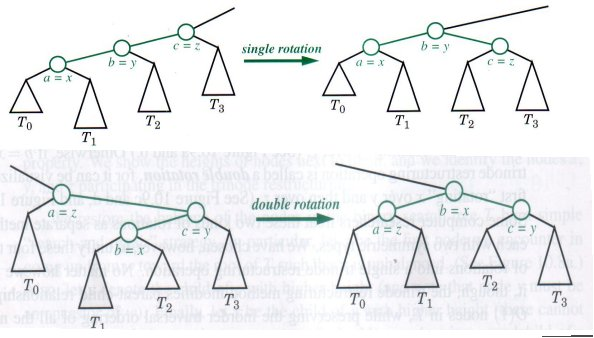
\includegraphics[scale=0.7]{equilibrage.jpg}
\caption{Méthodes d'équilibrages d'arbres AVL}
\label{avleq}
\end{figure}



\section*{Question 8 : Zacharie Kerger}
% add sections if more questions

\end{document}
